\documentclass[8pt]{beamer}

\useoutertheme{infolines}
\usecolortheme[rgb={0.65,0.15,0.25}]{structure}
\beamertemplatenavigationsymbolsempty
%\AtBeginSubsection

% Packages
\usepackage[latin1]{inputenc}
\usepackage{color}
\usepackage{xspace}
\usepackage{dsfont, stmaryrd}
\usepackage{amsmath, amsfonts, amssymb, stmaryrd}
\usepackage{epsfig}
\usepackage{tikz}
\usepackage{url}
\usepackage{/home/robin/LATEX/Biblio/astats}
\usepackage{graphicx}
\usepackage{xspace}

% Maths
% \newtheorem{theorem}{Theorem}
% \newtheorem{definition}{Definition}
\newtheorem{proposition}{Proposition}
% \newtheorem{assumption}{Assumption}
% \newtheorem{algorithm}{Algorithm}
% \newtheorem{lemma}{Lemma}
% \newtheorem{remark}{Remark}
% \newtheorem{exercise}{Exercise}
% \newcommand{\propname}{Prop.}
% \newcommand{\proof}{\noindent{\sl Proof:}\quad}
% \newcommand{\eproof}{$\blacksquare$}

% \setcounter{secnumdepth}{3}
% \setcounter{tocdepth}{3}
\newcommand{\pref}[1]{\ref{#1} p.\pageref{#1}}
\newcommand{\qref}[1]{\eqref{#1} p.\pageref{#1}}

% Colors : http://latexcolor.com/
\definecolor{darkred}{rgb}{0.65,0.15,0.25}
\definecolor{darkgreen}{rgb}{0,0.4,0}
\definecolor{darkred}{rgb}{0.65,0.15,0.25}
\definecolor{amethyst}{rgb}{0.6, 0.4, 0.8}
\definecolor{asparagus}{rgb}{0.53, 0.66, 0.42}
\definecolor{applegreen}{rgb}{0.55, 0.71, 0.0}
\definecolor{awesome}{rgb}{1.0, 0.13, 0.32}
\definecolor{blue-green}{rgb}{0.0, 0.87, 0.87}
\definecolor{red-ggplot}{rgb}{0.52, 0.25, 0.23}
\definecolor{green-ggplot}{rgb}{0.42, 0.58, 0.00}
\definecolor{purple-ggplot}{rgb}{0.34, 0.21, 0.44}
\definecolor{blue-ggplot}{rgb}{0.00, 0.49, 0.51}

% Commands
\newcommand{\backupbegin}{
   \newcounter{finalframe}
   \setcounter{finalframe}{\value{framenumber}}
}
\newcommand{\backupend}{
   \setcounter{framenumber}{\value{finalframe}}
}
\newcommand{\emphase}[1]{\textcolor{darkred}{#1}}
\newcommand{\comment}[1]{\textcolor{gray}{#1}}
\newcommand{\paragraph}[1]{\textcolor{darkred}{#1}}
\newcommand{\refer}[1]{{\small{\textcolor{gray}{{\cite{#1}}}}}}
\newcommand{\Refer}[1]{{\small{\textcolor{gray}{{[#1]}}}}}
\newcommand{\goto}[1]{{\small{\textcolor{blue}{[\#\ref{#1}]}}}}
\renewcommand{\newblock}{}

\newcommand{\tabequation}[1]{{\medskip \centerline{#1} \medskip}}
% \renewcommand{\binom}[2]{{\left(\begin{array}{c} #1 \\ #2 \end{array}\right)}}

% Variables 
\newcommand{\Abf}{{\bf A}}
\newcommand{\Beta}{\text{B}}
\newcommand{\Bcal}{\mathcal{B}}
\newcommand{\Bias}{\xspace\mathbb B}
\newcommand{\Cor}{{\mathbb C}\text{or}}
\newcommand{\Cov}{{\mathbb C}\text{ov}}
\newcommand{\cl}{\text{\it c}\ell}
\newcommand{\Ccal}{\mathcal{C}}
\newcommand{\cst}{\text{cst}}
\newcommand{\Dcal}{\mathcal{D}}
\newcommand{\Ecal}{\mathcal{E}}
\newcommand{\Esp}{\xspace\mathbb E}
\newcommand{\Espt}{\widetilde{\Esp}}
\newcommand{\Covt}{\widetilde{\Cov}}
\newcommand{\Ibb}{\mathbb I}
\newcommand{\Fcal}{\mathcal{F}}
\newcommand{\Gcal}{\mathcal{G}}
\newcommand{\Gam}{\mathcal{G}\text{am}}
\newcommand{\Hcal}{\mathcal{H}}
\newcommand{\Jcal}{\mathcal{J}}
\newcommand{\Lcal}{\mathcal{L}}
\newcommand{\Mt}{\widetilde{M}}
\newcommand{\mt}{\widetilde{m}}
\newcommand{\Nbb}{\mathbb{N}}
\newcommand{\Mcal}{\mathcal{M}}
\newcommand{\Ncal}{\mathcal{N}}
\newcommand{\Ocal}{\mathcal{O}}
\newcommand{\pt}{\widetilde{p}}
\newcommand{\Pt}{\widetilde{P}}
\newcommand{\Pbb}{\mathbb{P}}
\newcommand{\Pcal}{\mathcal{P}}
\newcommand{\Qcal}{\mathcal{Q}}
\newcommand{\qt}{\widetilde{q}}
\newcommand{\Rbb}{\mathbb{R}}
\newcommand{\Sbb}{\mathbb{S}}
\newcommand{\Scal}{\mathcal{S}}
\newcommand{\st}{\widetilde{s}}
\newcommand{\St}{\widetilde{S}}
\newcommand{\Tcal}{\mathcal{T}}
\newcommand{\todo}{\textcolor{red}{TO DO}}
\newcommand{\Ucal}{\mathcal{U}}
\newcommand{\Un}{\math{1}}
\newcommand{\Vcal}{\mathcal{V}}
\newcommand{\Var}{\mathbb V}
\newcommand{\Vart}{\widetilde{\Var}}
\newcommand{\Zcal}{\mathcal{Z}}

% Symboles & notations
\newcommand\independent{\protect\mathpalette{\protect\independenT}{\perp}}\def\independenT#1#2{\mathrel{\rlap{$#1#2$}\mkern2mu{#1#2}}} 
\renewcommand{\d}{\text{\xspace d}}
\newcommand{\gv}{\mid}
\newcommand{\ggv}{\, \| \, }
% \newcommand{\diag}{\text{diag}}
\newcommand{\card}[1]{\text{card}\left(#1\right)}
\newcommand{\trace}[1]{\text{tr}\left(#1\right)}
\newcommand{\matr}[1]{\boldsymbol{#1}}
\newcommand{\matrbf}[1]{\mathbf{#1}}
\newcommand{\vect}[1]{\matr{#1}} %% un peu inutile
\newcommand{\vectbf}[1]{\matrbf{#1}} %% un peu inutile
\newcommand{\trans}{\intercal}
\newcommand{\transpose}[1]{\matr{#1}^\trans}
\newcommand{\crossprod}[2]{\transpose{#1} \matr{#2}}
\newcommand{\tcrossprod}[2]{\matr{#1} \transpose{#2}}
\newcommand{\matprod}[2]{\matr{#1} \matr{#2}}
\DeclareMathOperator*{\argmin}{arg\,min}
\DeclareMathOperator*{\argmax}{arg\,max}
\DeclareMathOperator{\sign}{sign}
\DeclareMathOperator{\tr}{tr}
\newcommand{\ra}{\emphase{$\rightarrow$} \xspace}

% Hadamard, Kronecker and vec operators
\DeclareMathOperator{\Diag}{Diag} % matrix diagonal
\DeclareMathOperator{\diag}{diag} % vector diagonal
\DeclareMathOperator{\mtov}{vec} % matrix to vector
\newcommand{\kro}{\otimes} % Kronecker product
\newcommand{\had}{\odot}   % Hadamard product

% TikZ
\newcommand{\nodesize}{2em}
\newcommand{\edgeunit}{2.5*\nodesize}
\newcommand{\edgewidth}{1pt}
\tikzstyle{node}=[draw, circle, fill=black, minimum width=.75\nodesize, inner sep=0]
\tikzstyle{square}=[rectangle, draw]
\tikzstyle{param}=[draw, rectangle, fill=gray!50, minimum width=\nodesize, minimum height=\nodesize, inner sep=0]
\tikzstyle{hidden}=[draw, circle, fill=gray!50, minimum width=\nodesize, inner sep=0]
\tikzstyle{hiddenred}=[draw, circle, color=red, fill=gray!50, minimum width=\nodesize, inner sep=0]
\tikzstyle{observed}=[draw, circle, minimum width=\nodesize, inner sep=0]
\tikzstyle{observedred}=[draw, circle, minimum width=\nodesize, color=red, inner sep=0]
\tikzstyle{eliminated}=[draw, circle, minimum width=\nodesize, color=gray!50, inner sep=0]
\tikzstyle{empty}=[draw, circle, minimum width=\nodesize, color=white, inner sep=0]
\tikzstyle{blank}=[color=white]
\tikzstyle{nocircle}=[minimum width=\nodesize, inner sep=0]

\tikzstyle{edge}=[-, line width=\edgewidth]
\tikzstyle{edgebendleft}=[-, >=latex, line width=\edgewidth, bend left]
\tikzstyle{edgebendright}=[-, >=latex, line width=\edgewidth, bend right]
\tikzstyle{lightedge}=[-, line width=\edgewidth, color=gray!50]
\tikzstyle{lightedgebendleft}=[-, >=latex, line width=\edgewidth, bend left, color=gray!50]
\tikzstyle{lightedgebendright}=[-, >=latex, line width=\edgewidth, bend right, color=gray!50]
\tikzstyle{edgered}=[-, line width=\edgewidth, color=red]
\tikzstyle{edgebendleftred}=[-, >=latex, line width=\edgewidth, bend left, color=red]
\tikzstyle{edgebendrightred}=[-, >=latex, line width=\edgewidth, bend right, color=red]

\tikzstyle{arrow}=[->, >=latex, line width=\edgewidth]
\tikzstyle{arrowbendleft}=[->, >=latex, line width=\edgewidth, bend left]
\tikzstyle{arrowbendright}=[->, >=latex, line width=\edgewidth, bend right]
\tikzstyle{arrowred}=[->, >=latex, line width=\edgewidth, color=red]
\tikzstyle{arrowbendleftred}=[->, >=latex, line width=\edgewidth, bend left, color=red]
\tikzstyle{arrowbendrightred}=[->, >=latex, line width=\edgewidth, bend right, color=red]
\tikzstyle{arrowblue}=[->, >=latex, line width=\edgewidth, color=blue]
\tikzstyle{dashedarrow}=[->, >=latex, dashed, line width=\edgewidth]
\tikzstyle{dashededge}=[-, >=latex, dashed, line width=\edgewidth]
\tikzstyle{dashededgebendleft}=[-, >=latex, dashed, line width=\edgewidth, bend left]
\tikzstyle{lightarrow}=[->, >=latex, line width=\edgewidth, color=gray!50]

\newcommand{\GMSBM}{/home/robin/RECHERCHE/RESEAUX/EXPOSES/1903-SemStat/}
\newcommand{\figeconet}{/home/robin/RECHERCHE/ECOLOGIE/EXPOSES/1904-EcoNet-Lyon/Figs}
\newcommand{\fignet}{/home/robin/RECHERCHE/RESEAUX/EXPOSES/FIGURES}
\newcommand{\figeco}{/home/robin/RECHERCHE/ECOLOGIE/EXPOSES/FIGURES}
\newcommand{\figbayes}{/home/robin/RECHERCHE/BAYES/EXPOSES/FIGURES}
\newcommand{\figCMR}{/home/robin/Bureau/RECHERCHE/ECOLOGIE/CountPCA/sparsepca/Article/Network_JCGS/trunk/figs}
\newcommand{\figDoR}{/home/robin/RECHERCHE/BAYES/VBEM-IS/VBEM-IS.git/Paper/JRSSC-V3/Figs}
\newcommand{\figlux}{./Figures}

\renewcommand{\nodesize}{1.75em}
\renewcommand{\edgeunit}{2.25*\nodesize}

%====================================================================
%====================================================================
\begin{document}
%====================================================================
%====================================================================
\title{4 - Beyond variational inference}

\author[S. Robin]{S. Robin \\ ~\\
  {\small INRAE / AgroParisTech / univ. Paris-Saclay \\
  Mus\'eum National d'Histoire Naturelle}
  }

\date[Luxembourg, Dec'20]{Winter School on Mathematical Statistics, Luxembourg, Dec'20}

\maketitle

%====================================================================
% Road map
\frame{\includegraphics{\figlux/RoadMap}}

%====================================================================
\frame{\frametitle{Part 4} \tableofcontents}

%====================================================================
%====================================================================
\section{Algorithmic improvements}
\frame{\frametitle{Outline} \tableofcontents[currentsection]}
%====================================================================
\frame{\frametitle{Algorithmic improvements} 

  \paragraph{Borrowed from many fields.}
  \begin{itemize}
  \item \bigskip Optimization: generic stochastic gradient descent \textcolor{gray}{(\#\ref{goto:reparmTrick})} or more dedicated approaches \refer{HBW13} \label{back:reparmTrick}
  \item \bigskip Bayesian inference: Variational tempering \refer{MMA16}
  \item \bigskip Machine learning: Variational autoencoders \refer{KiW14,KiW19} \\
  \bigskip 
  \ra use neural networks to learn the variational parameters with more flexibility
  \end{itemize}

}
  


%====================================================================
%====================================================================
\section{Guaranties about variational estimates}
\frame{\frametitle{Outline} \tableofcontents[currentsection]}
%====================================================================
\frame{\frametitle{Statistical guarantees: \emphase{\sl no big picture}} 

  \bigskip 
  \paragraph{Accuracy of variational estimates.}
  \begin{itemize}
  \item Most often assessed empirically (numerical simulations) \textcolor{gray}{see e.g. \#\ref{goto:vbemSBM}} \label{back:vbemSBM}
%   \item Theoretical guarantees: 
  \end{itemize}

  \pause \bigskip \bigskip 
  \paragraph{'Negative' results.}
  \begin{itemize}
  \item VEM estimates $\neq$ stationary point of the likelihood function \refer{GuB05}
  \item Too small posterior variance provided by variational Bayes \refer{WaT05,McT07,CoM07}
  \end{itemize}

  \pause \bigskip \bigskip 
  \paragraph{Balanced results.}
  \begin{itemize}
  \item Mean-field approximation provides consistent estimates (binary SBM affiliation: \refer{ZhZ20})
  \item Naive implementation may yield instabilities \refer{GJM19,ZhZ20}
  \end{itemize}

  \pause \bigskip \bigskip 
  \paragraph{Positive results.}
  \begin{itemize}
  \item Some results for specific models \refer{HOW11}
  \item Some attempts for a general theory via $M$-estimation \refer{WeM19}
  \item Most studied case: mean-field VEM binary stochastic block-model (see next)
  \end{itemize}

%  Model selection

}
  
%====================================================================
\frame{\frametitle{Binary stochastic block-model} 

  \paragraph{A series of results:} \refer{CDP12,BCC13,MaM15,ZhZ20} 
  \begin{itemize}
  \item Consistency of variational estimates
  \item Asymptotic normality of variational estimates
  \item Class recovery (node classification, including LBM)
  \end{itemize}

  \pause \bigskip \bigskip 
  \paragraph{Why does it work?} Theorem 3.1 in \refer{CDP12} states that
  $$
  P\left(\sum_{z \neq z^*} \frac{p_\theta(Z=z \mid Y)}{p_\theta(Z=z^* \mid Y)} > t \right) = O\left(n e^{-\kappa n t}\right)
  $$
  uniformly in $z^*$, with $\kappa = \kappa(\theta)$.

  \pause \bigskip \bigskip 
  \begin{itemize}
  \item Intuition: $p_\theta(Z \mid Y)$ is asymptotically Dirac, which belongs to $\Qcal = \Qcal_{fact}$.
  \item The 'largest gap' algorithm \refer{CDR12} takes advantage of a similar concentration \textcolor{gray}{\#\ref{goto:largestGap}} \label{back:largestGap}
  \item The proofs do not easily adapt to other VEM
  \end{itemize}

}
  


%====================================================================
%====================================================================
\section{Combining variational inference with ...}
\frame{\frametitle{Outline} \tableofcontents[currentsection]}
%====================================================================
\subsection{Frequentist inference}
%====================================================================
\frame{\frametitle{Frequentist inference} \pause

  \paragraph{Maximum likelihood inference.}
  $$
  \widehat{\theta}_{MLE} = \argmax_\theta \; \log p_\theta(Y)
  $$
  is intractable because the likelihood involves an integration over the latent $Z$
  \begin{align*}
  \text{PLN:} \qquad 
  \log p_\theta(Y) & = \sum_i \log \left(\emphase{\int_{\Rbb^p}} p_\Sigma(Z_i) \prod_j p_\beta(Y_{ij} \mid Z_{ij}) \d Z_i \right) \\
  ~ \\
  \text{SBM:} \qquad 
  \log p_\theta(Y) & = \log \left(\emphase{\sum_{Z \in [K]^n}} \prod_i p_\pi(Z_i) \prod_{i, j} p_{\alpha, \beta}(Y_{ij} \mid Z_i, Z_j) \right) 
  \end{align*}
  
  \pause \bigskip \bigskip
  The (log-)likelihood is far from being the only admissible estimation function \\
  ~ \\
  \ra think, e.g., of $M$-estimation

}
  
%====================================================================
\frame{\frametitle{Composite likelihood} 

  \paragraph{Sum of partial likelihoods:} 
  \begin{align*}
  \text{PLN:} \qquad 
  \widehat{\theta}_{CL} 
  & = \argmax_\theta \; \sum_i \sum_{j, k} \log p_\theta(Y_{ij}, Y_{ik}) &
  & \text{only requires $\int_{\Rbb^2}$} \\
  ~ \\
  \text{SBM:} \qquad 
  \widehat{\theta}_{CL} 
  & = \argmax_\theta \; \sum_{i, j, k} \log p_\theta(Y_{ij}, Y_{ik}, Y_{jk}) &
  & \text{only requires $\sum_{Z \in [K]^3}$} \\
  \end{align*}
  \ra Generic results (consistency, asymptotic normality) exist for $\widehat{\theta}_{CL}$ \refer{VRF11} +  see \refer{AmM12} for binary SBM
  
  \pause \bigskip \bigskip 
  \paragraph{Practical implementation.}
  \begin{itemize}
  \item EM algorithms can be designed to maximize composite likelihoods
  \item \bigskip Getting $\widehat{\theta}_{CL}$ is still demanding (many terms in the sum: $np^2$ for PLN, $n^3$ for SBM)
  \item \bigskip $\widehat{\theta}_{VEM}$ usually provides a (very) good starting point
  \end{itemize}


}
  
%====================================================================
\subsection{Bayesian inference}
%====================================================================
\frame{\frametitle{Bayesian inference} \pause

  \paragraph{Reminder.}
  \begin{itemize}
  \item Prior: $p(\theta)$ \qquad \qquad \qquad \textcolor{gray}{$\theta_{PLN} = (\beta, \Sigma)$, \quad $\theta_{SBM} = (\pi, \alpha, \beta)$}
  \item Latent: $p(Z \mid \theta)$
  \item Observed: $p(Y \mid Z, \theta)$
  \item Posterior:
  $$
  p(\theta, Z \mid Y) = \frac{p(\theta) \; p(Z \mid \theta) \; p(Y \mid, \theta, Z)}{p(Y)}
  $$
  \end{itemize}

  \pause \bigskip 
  \paragraph{Sampling methods.}
  \begin{itemize}
  \item \pause Monte-Carlo: sample $(\theta^b, Z^b) \overset{\text{iid}}{\sim} p(\theta, Z \mid Y)$
  \item \pause MCMC: construct a Markov chain with $p(\theta, Z \mid Y)$ as a stationary distribution
  \item \pause Importance sampling: $(\theta^b, Z^b) \overset{\text{iid}}{\sim} q(\theta, Z )$ and reweight each draw with weight
  $$
  w^b = \frac{p(\theta^b, Z^b \mid Y)}{q(\theta^b, Z^b)}
  $$
  \item \pause Sequential Monte-Carlo: construct a sequence of distribution going from $q(\theta, Z )$ to $p(\theta, Z \mid Y)$
  \end{itemize}

}

%====================================================================
\frame{\frametitle{Sequential Monte-Carlo sampling} 

  \begin{tabular}{cc}
    \hspace{-.04\textwidth}
    \begin{tabular}{p{.5\textwidth}} 
      \paragraph{Principle.} \refer{DDJ06} $U = (\theta, Z)$ \\ ~ 
      \begin{itemize}
        \item \pause given $\textcolor{blue}{p_{{start}}(U)}$ \\ ~ 
        \item \pause aiming at $\textcolor{red}{p_{{target}}(U)} =  p(U \mid Y)$ \\ ~
        \item \pause sample from a sequence of distributions
%         $p_{\text{start}} = p_0$, $p_1$, $\dots$, $p_{H-1}$, $p_H = p_{\text{target}}$
        $$
        \textcolor{blue}{p_{{start}} = p_0}, \; p_1, \; \dots, \; p_{H-1}, \; \textcolor{red}{p_H = p_{{target}}}
        $$
        with
        $$
        p_h(U) \propto p_{{start}}(U)^{{1 - \rho_h}} p_{{target}}(U)^{{\rho_h}}
        $$
        and $0 = \rho_0 < \rho_1 \ < \dots < \rho_H = 1$
      \end{itemize}
    \end{tabular}
    &
    \begin{tabular}{p{.45\textwidth}}
      \includegraphics[width=.4\textwidth]{\figbayes/FigVBEM-IS-Tempering-4to2} \\
      \textcolor{gray}{see \#\ref{goto:SMC} for tuning of the $\rho_h$} \label{back:SMC}
    \end{tabular}
  \end{tabular}
  
  \pause \bigskip 
  \begin{description}
  \item[Most often:] $p_{{start}} = p_{prior}$ \qquad (long way to the posterior)
  \item[VBEM:] \smallskip directly use $p_{{start}} = p_{VBEM}$
  \item[VEM:] \smallskip use (approximate) Louis formulas \refer{Lou82} to derive $p_{{start}} = p_{VEM}$ \refer{DoR19}
  \end{description}

  
} 

%====================================================================
\frame{\frametitle{Back to the tree interaction network} 

  \begin{tabular}{ccc}
    \hspace{-.04\textwidth}
    \begin{tabular}{p{.35\textwidth}}
      $$
      \begin{array}{rl}
      Y_{ij} & = \text{number of shared parasites} \\
      x_{ij} & = \text{taxonomic distance} \\
      Y_{ij} & \sim \Pcal(\exp(x_{ij}^\intercal \beta + \alpha_{Z_iZ_j}))
      \end{array}
      $$
      ~ \\

      \paragraph{Estimates:}
      $$
      \widehat{K}_{ICL} = 4
      \qquad 
      \widehat{\beta} = -.317
      $$
      {\begin{itemize}
      \item Taxonomy (partially) explains the links (smaller $\widehat{K}$)
      \item \bigskip Distant species share less parasites ($\widehat{\beta} < 0$)
      \item \bigskip The remaining structure is \emphase{not related to taxonomy}
      \end{itemize}}
    \end{tabular}
    &
    \hspace{-.05\textwidth}
    \begin{tabular}{p{.3\textwidth}}
      \paragraph{No covariate:} $\widehat{K}_{ICL} = 7$ \\
      \includegraphics[height=.3\textwidth, width=.3\textwidth]{\fignet/Tree-adjMat-SBMnull} \\
      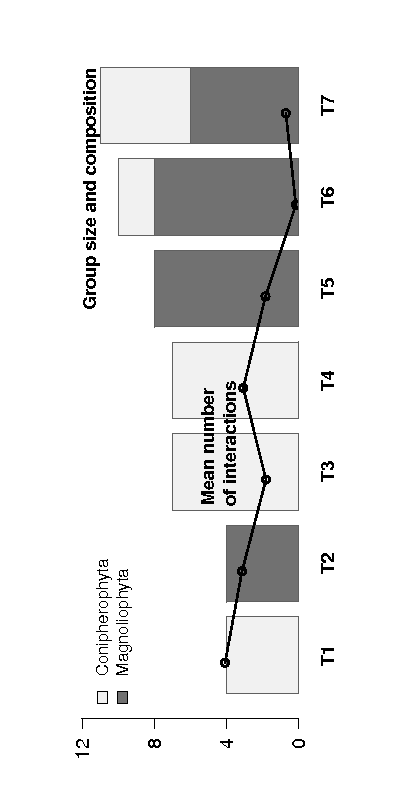
\includegraphics[height=.3\textwidth, width=.3\textwidth, trim=150 150 150 150]{\fignet/MRV10_AoAS_Q7_group}
    \end{tabular}
    &
    \hspace{-.05\textwidth}
    \begin{tabular}{p{.3\textwidth}}
      \paragraph{Taxonomic dist.:} $\widehat{K}_{ICL} = 4$ \\
      \includegraphics[height=.3\textwidth, width=.3\textwidth]{\fignet/Tree-adjMat-SBMtaxo} \\
      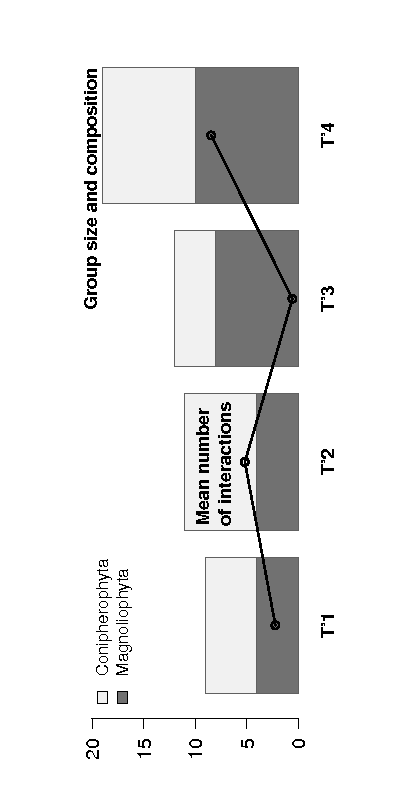
\includegraphics[height=.3\textwidth, width=.3\textwidth, trim=150 150 150 150]{\fignet/MRV10_AoAS_Q4_group}
    \end{tabular}
  \end{tabular}

}

%====================================================================
\frame{\frametitle{Tree network: model selection} 

  \paragraph{Model selection.} 
  \begin{itemize}
  \item Number of groups $K$ 
  \item Set $S$ of relevent covariates: $S \subset \{\text{taxonomy, geography, phylogeny}\}$
  \end{itemize}
  
  \pause \bigskip 
  \begin{tabular}{ccc}
    \hspace{-.04\textwidth}
    \begin{tabular}{p{.4\textwidth}}
      \paragraph{Choosing $K$} for a given $S$:
      $$
      p(K \mid Y, S) \propto p(Y \mid S, K)
      $$
      here : $S = (\text{taxonomy, geography})$ \\
      ~ \\ 
      \textcolor{gray}{Averaging over $K$: \#\ref{goto:graphon}} \label{back:graphon} \\
      ~ \\
    \end{tabular}
    &
    \begin{tabular}{p{.3\textwidth}}
      \includegraphics[width=.25\textwidth]{\figDoR/Tree-all-V10-M5000-logpY}
    \end{tabular}
    &
    \hspace{-.1\textwidth}
    \begin{tabular}{p{.2\textwidth}}
      $\log p(Y \mid S, K)$ \\ ~ \\
      \textcolor{blue}{$J_{\widehat{\theta}, \widehat{q}}$} \\ ~ \\
      \textcolor{red}{$vICL$} \\ 
    \end{tabular}
  \end{tabular}
  
  \pause \bigskip \bigskip 
  \paragraph{Variable selection.} $p(S \mid Y) = \sum_K p(S, K \mid Y)$
  $$
  P\{x = \text{(taxo., geo.)} \mid Y \} \simeq 70\%, \qquad
  P\{x = \text{(taxo.)} \mid Y \} \simeq 30\%
  $$

}

%====================================================================
\frame{\frametitle{Tree network: significance} 

  \paragraph{Parameter posterior distribution} for $S = (\text{taxonomy, geography, phylogeny})$: 
  $$
  \begin{array}{ccc}
    \text{taxonomy} & \text{geography} & \text{phylogeny} \\
    \includegraphics[width=.25\textwidth]{\figDoR/Tree-all-V10-M5000-beta1} & 
    \includegraphics[width=.25\textwidth]{\figDoR/Tree-all-V10-M5000-beta2} & 
    \includegraphics[width=.25\textwidth]{\figDoR/Tree-all-V10-M5000-beta3} \\
    \multicolumn{3}{l}{\text{Legend:} \qquad 
      \textcolor{blue}{q_{VEM}(\beta_j)}, \qquad 
      \textcolor{red}{p(\beta_j \mid S, \widehat{K}(S), Y)}, \qquad 
      p(\beta_j \mid S, Y) }
  \end{array}
  $$
  
  \bigskip \pause
  \paragraph{Why so many steps} to go from \textcolor{blue}{$q_{VEM}(\beta_j)$} to \textcolor{red}{$p(\beta_j \mid Y)$} ?
  
  \bigskip 
  \hspace{-.025\textwidth}
  \begin{tabular}{rrrr}
    \paragraph{Correlation between estimates.} 
    & $(\beta_1, \beta_2)$ & $(\beta_1, \beta_3)$ & $(\beta_2, \beta_3)$ \\
    $p_{VEM}(\beta)$    & $-0.012$ & $ 0.021$ & $ 0.318$ \\
    $p(\beta \mid Y)$ & $-0.274$ & $-0.079$ & $-0.088$
  \end{tabular}
  
  \bigskip
  \textcolor{gray}{+ $p(Z \mid Y)$ in \#\ref{goto:smcPath}} \label{back:smcPath}

}


%====================================================================
%====================================================================
\section{Conclusion (?)}
\frame{\frametitle{Outline} \tableofcontents[currentsection]}
%====================================================================
\frame{\frametitle{Conclusion} 

  \paragraph{Latent variable models (in ecology).}
  \begin{itemize}
  \item Very useful (hope you're convinced) 
  \end{itemize}

  \bigskip \bigskip 
  \paragraph{Variational inference (computational side).}
  \begin{itemize}
  \item Computationally efficient
  \item Reasonably easy to implement (hope you're convinced too)
  \end{itemize}
  
  \bigskip \bigskip 
  \paragraph{Variational inference (theoretical side).}
  \begin{itemize}
  \item Generic analysis of variational estimation still to do
  \item Alternatively: combine with other inference methods to combine computational efficiency with pre-existing statistical guarantees
  \end{itemize}

}



%====================================================================
%====================================================================
\backupbegin 
\section*{Backup}
%====================================================================
\frame[allowframebreaks]{ \frametitle{References}
  {\tiny
   \bibliography{/home/robin/Biblio/BibGene}
   \bibliographystyle{alpha}
  }
}

%====================================================================
%====================================================================
\section*{Backup}
%====================================================================
\frame{\frametitle{Reparametrization trick} \label{goto:reparmTrick}

  Denoting by $\psi$ the variational parameter, The VE step aims at minimizing
  $$
  KL[q_\psi(Z) \| p_\theta(Z \mid Y)] = \Esp_{q_\psi} \log \frac{q_\psi(Z)}{p_\theta(Z \mid Y)}
  $$
  
  \bigskip 
  Stochastic gradient descent requires an unbiased estimate of the gradient $\nabla_\psi \Esp_{q_\psi} (\cdot)$ ... \\
  which is {\sl not} provided by sampling $Z^b \overset{\text{iid}}{\sim} q_\psi$ to estimate $\Esp_{q_\psi}$.

  \bigskip \bigskip 
  \paragraph{Trick \refer{KiW14,KiW19}.}
  Suppose there exist a fix distribution $q^0$ and a function $f$, such that\footnote{Think of $q^0 = \Ncal(0, I)$, $\psi = (\mu, \Sigma)$, $q_\psi = \Ncal(\mu, \Sigma)$.}
  $$
  \epsilon \sim q^0 
  \qquad \Rightarrow \qquad Z = f(\epsilon, \psi) \sim q_\psi, 
  $$
  Then, sampling $\epsilon^b \overset{\text{iid}}{\sim} q^0$ provides an unbiased estimate of the gradient:
  $$
  \nabla_\psi \; \Esp_{q_\psi} \log \frac{q_\psi(Z)}{p_\theta(Z \mid Y)}
  \simeq 
  \nabla_\psi \; \left( \frac1B \sum_b \log \frac{q_\psi(f(\epsilon^b, \psi))}{p_\theta(f(\epsilon^b, \psi) \mid Y)} \right)
  $$

  \textcolor{gray}{Back to \#\ref{back:reparmTrick}}

}

%====================================================================
\frame{\frametitle{VBEM for binary SBM}  \label{goto:vbemSBM}

  \paragraph{Posterio credibility intervals (CI) \refer{GDR12}:}  
  Actual level for $\pi_1$ ($+$), $\gamma_{11}$
  (\textcolor{red}{$\triangle$}), $\gamma_{12}$
  (\textcolor{blue}{$\circ$}), $\gamma_{22}$
  (\textcolor{green}{$\bullet$}) \\
  \includegraphics[width=.9\textwidth]{\fignet/im-ICQ2-2-new} \\
%   \pause \ra For all parameters, {\VBEM} posterior credibility
%   intervals achieve the nominal level (90\%), as soon as $n \geq 30$.

  \emphase{Width of the posterior CI.}
  {$\pi_1$}, \textcolor{red}{$\gamma_{11}$},
  \textcolor{blue}{$\gamma_{12}$}, \textcolor{green}{$\gamma_{22}$}
  \\
  \includegraphics[width=1\textwidth]{\fignet/im-ICQ2-3} \\

  \bigskip
  \ra 
  Width $\approx 1/\sqrt{n}$ for $\pi_1$ and $\approx 1/n = 1/\sqrt{n^2}$ for $\gamma_{11}$, $\gamma_{12}$ and $\gamma_{22}$.

  \bigskip
  \textcolor{gray}{Back to \#\ref{back:vbemSBM}}

}

%====================================================================
\frame{\frametitle{Largest gap algorithm} \label{goto:largestGap}

  \begin{tabular}{cc}
    \hspace{-.04\textwidth}
    \begin{tabular}{p{.45\textwidth}}
      \begin{itemize}
      \item \emphase{Degree} of a node: $D_i = \sum_{j \neq i} Y_{ij}$
      \item \bigskip Mean connection from group $k$:
      $$
      \overline{\gamma}_k = \sum_\ell \pi_\ell \gamma_{k\ell}
      $$
      \item \bigskip Degree distribution\footnote{Balanced affiliation model = nasty case: $\pi_k \equiv 1/K, \gamma_{kk} = \gamma_{in}, \gamma_{k\ell} = \gamma_{out} \quad \Rightarrow \quad  \overline{\gamma}_k \equiv (\gamma_{in} + (K-1)\gamma_{out})/K$}
      $$
      (D_i \mid Z_i = k) \sim \Bcal(n-1, \overline{\gamma}_k)
      $$
      \item \bigskip \emphase{Concentration} of $D_i / (n-1)$ around $\overline{\gamma}_{Z_i}$ at exponential rate 
      \end{itemize}
    \end{tabular}
    &
    \hspace{-.05\textwidth}
    \begin{tabular}{p{.45\textwidth}}
      \includegraphics[height=.7\textheight]{\fignet/FigLargestGap-Histograms}
    \end{tabular}
  \end{tabular}
  
  \ra Ensures consistency \refer{CDR12} (including sparse regime)  
  
  \bigskip
  \textcolor{gray}{Back to \#\ref{back:largestGap}}

}
  
%====================================================================
\frame{\frametitle{Sequential importance sampling scheme} \label{goto:SMC}

  Consider $\emphase{U = (\theta, Z)}$
  
  \bigskip
  \paragraph{Distribution path:}
    set $0 = \rho_0 < \rho_1 < \dots < \rho_{H-1} < \rho_H = 1$,
  \begin{align*}
     p_h(U) & \propto p_{\text{start}}(U)^{\emphase{{1-\rho_h}}} \; \times \; p_{\text{target}}(U)^{\emphase{{\rho_h}}} \\
     \\
     & \propto p_{\text{start}}(U) \; \times \; r(U)^{\emphase{{\rho_h}}}, 
     & r(U) & = \frac{p(U) p(Y \mid U)}{p_{\text{start}}(U)}
  \end{align*}
  
  \bigskip \bigskip \pause
  \paragraph{Sequential sampling.} At each step $h$, provides
  $$
  \Ecal_h = \{(U_h^m, w_h^m)\}_m = \text{ weighted sample of } p_h
  $$

  \bigskip \pause
  \paragraph{Tune $\rho_{h+1}$} 
  to keep the efficient sample size sufficiently high at each step. \\
  ~ \\
  \ra Doable because $r(U)$ does not depend on $\rho$.

}

%====================================================================
\frame{\frametitle{Sequential sampling: in pictures}  

  \begin{tabular}{cc}
    \hspace{-.04\textwidth}
   \begin{tabular}{p{.5\textwidth}}
      \begin{itemize}
        \onslide+<1->{\item $\textcolor{blue}{p_{\text{start}}} = $ proposal, $\textcolor{red}{p_{\text{target}}} = $ target \\ ~ \\} 
        \onslide+<2->{\item Intermediate distributions
        $p_{\text{start}} = p_0$, $p_1$, $...$, $p_H = p_{\text{target}}$ \\ ~ \\}
        \onslide+<3->{\item Iteratively: \\
        use $p_h$ to get a sample from $p_{h+1}$}
      \end{itemize}
    \end{tabular}
    & 
    \hspace{-.02\textwidth}
    \begin{tabular}{p{.5\textwidth}}
      \begin{overprint}
        \onslide<1> 
        \includegraphics[width=.4\textwidth]{\figbayes/FigVBEM-IS-PropTarget-4to2}
        \onslide<2> 
        \includegraphics[width=.4\textwidth]{\figbayes/FigVBEM-IS-Tempering-4to2}
        \onslide<3> 
        \includegraphics[width=.4\textwidth]{\figbayes/FigVBEM-IS-Tempering-step1-4to2}
        \onslide<4> 
        \includegraphics[width=.4\textwidth]{\figbayes/FigVBEM-IS-Tempering-step2-4to2}
        \onslide<5> 
        \includegraphics[width=.4\textwidth]{\figbayes/FigVBEM-IS-Tempering-step3-4to2}
        \onslide<6-> 
        \includegraphics[width=.4\textwidth]{\figbayes/FigVBEM-IS-Tempering-step4-4to2}
      \end{overprint}
    \end{tabular}
  \end{tabular}  
  
  \bigskip
  \onslide+<7>{+ resampling/propagation to avoid complete degeneracy \refer{DoR19}}

  \bigskip
  \textcolor{gray}{Back to \#\ref{back:SMC}}

}

%====================================================================
\frame{\frametitle{Residual 'graphon'} \label{goto:graphon}

  \paragraph{Graphon representation of $(\pi, \alpha)$.} \refer{LaR16,DoR19}
  \begin{align*}
    \phi_K: (0, 1) \times (0, 1) \mapsto \Rbb
    \qquad \text{block wise constant} 
  \end{align*}
  For a given set $S$, averaging over $K$ gives
  $$
  \widehat{\phi}(u, v) 
  = \Esp \left(\phi_K(u, v) \mid Y, S\right)
  = \sum_K p(K \mid Y, S) \Esp \left(\phi_K(u, v) \mid Y, S, K\right)
  $$

  \pause \bigskip \bigskip
  $$
  \begin{array}{ccc}
    \text{SBM graphon} & \text{$\widehat{\phi}$ for the tree network} & \text{$U_i$ vs nb. neighbors} \\
    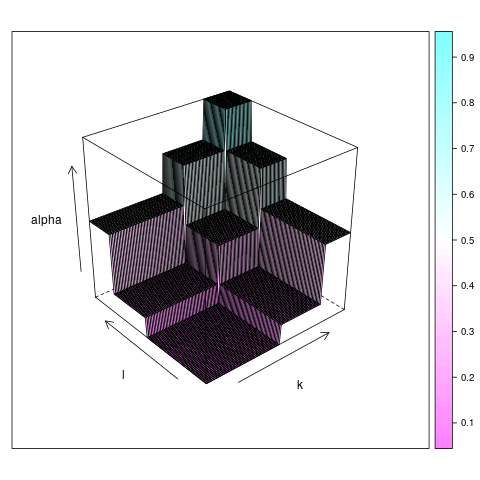
\includegraphics[trim=60 60 60 60, width=.25\textwidth]{\figDoR/FigGraphon-SBM-graphon-alpha} &
    \includegraphics[trim=60 60 60 60, width=.25\textwidth]{\figDoR/Tree-all-V10-M5000-graphon} &
    \includegraphics[width=.25\textwidth]{\figDoR/Tree-all-V10-M5000-Ui-neighbours} 
  \end{array}
  $$
  
  \bigskip
  \textcolor{gray}{Back to \#\ref{back:graphon}}
  
}

%====================================================================
\frame{\frametitle{SMC path} \label{goto:smcPath}

  $$
  \begin{array}{cc|c}
    \multicolumn{2}{c|}{\text{Tree network, $S = \{taxo., geo.\}$}}
    &  \text{Simulations} \\
    & & \\
    \hline
    \includegraphics[width=.25\textwidth]{\figDoR/Tree-all-V10-M5000-rho} & 
    \includegraphics[width=.25\textwidth]{\figDoR/Tree-all-V10-M5000-MI} &
    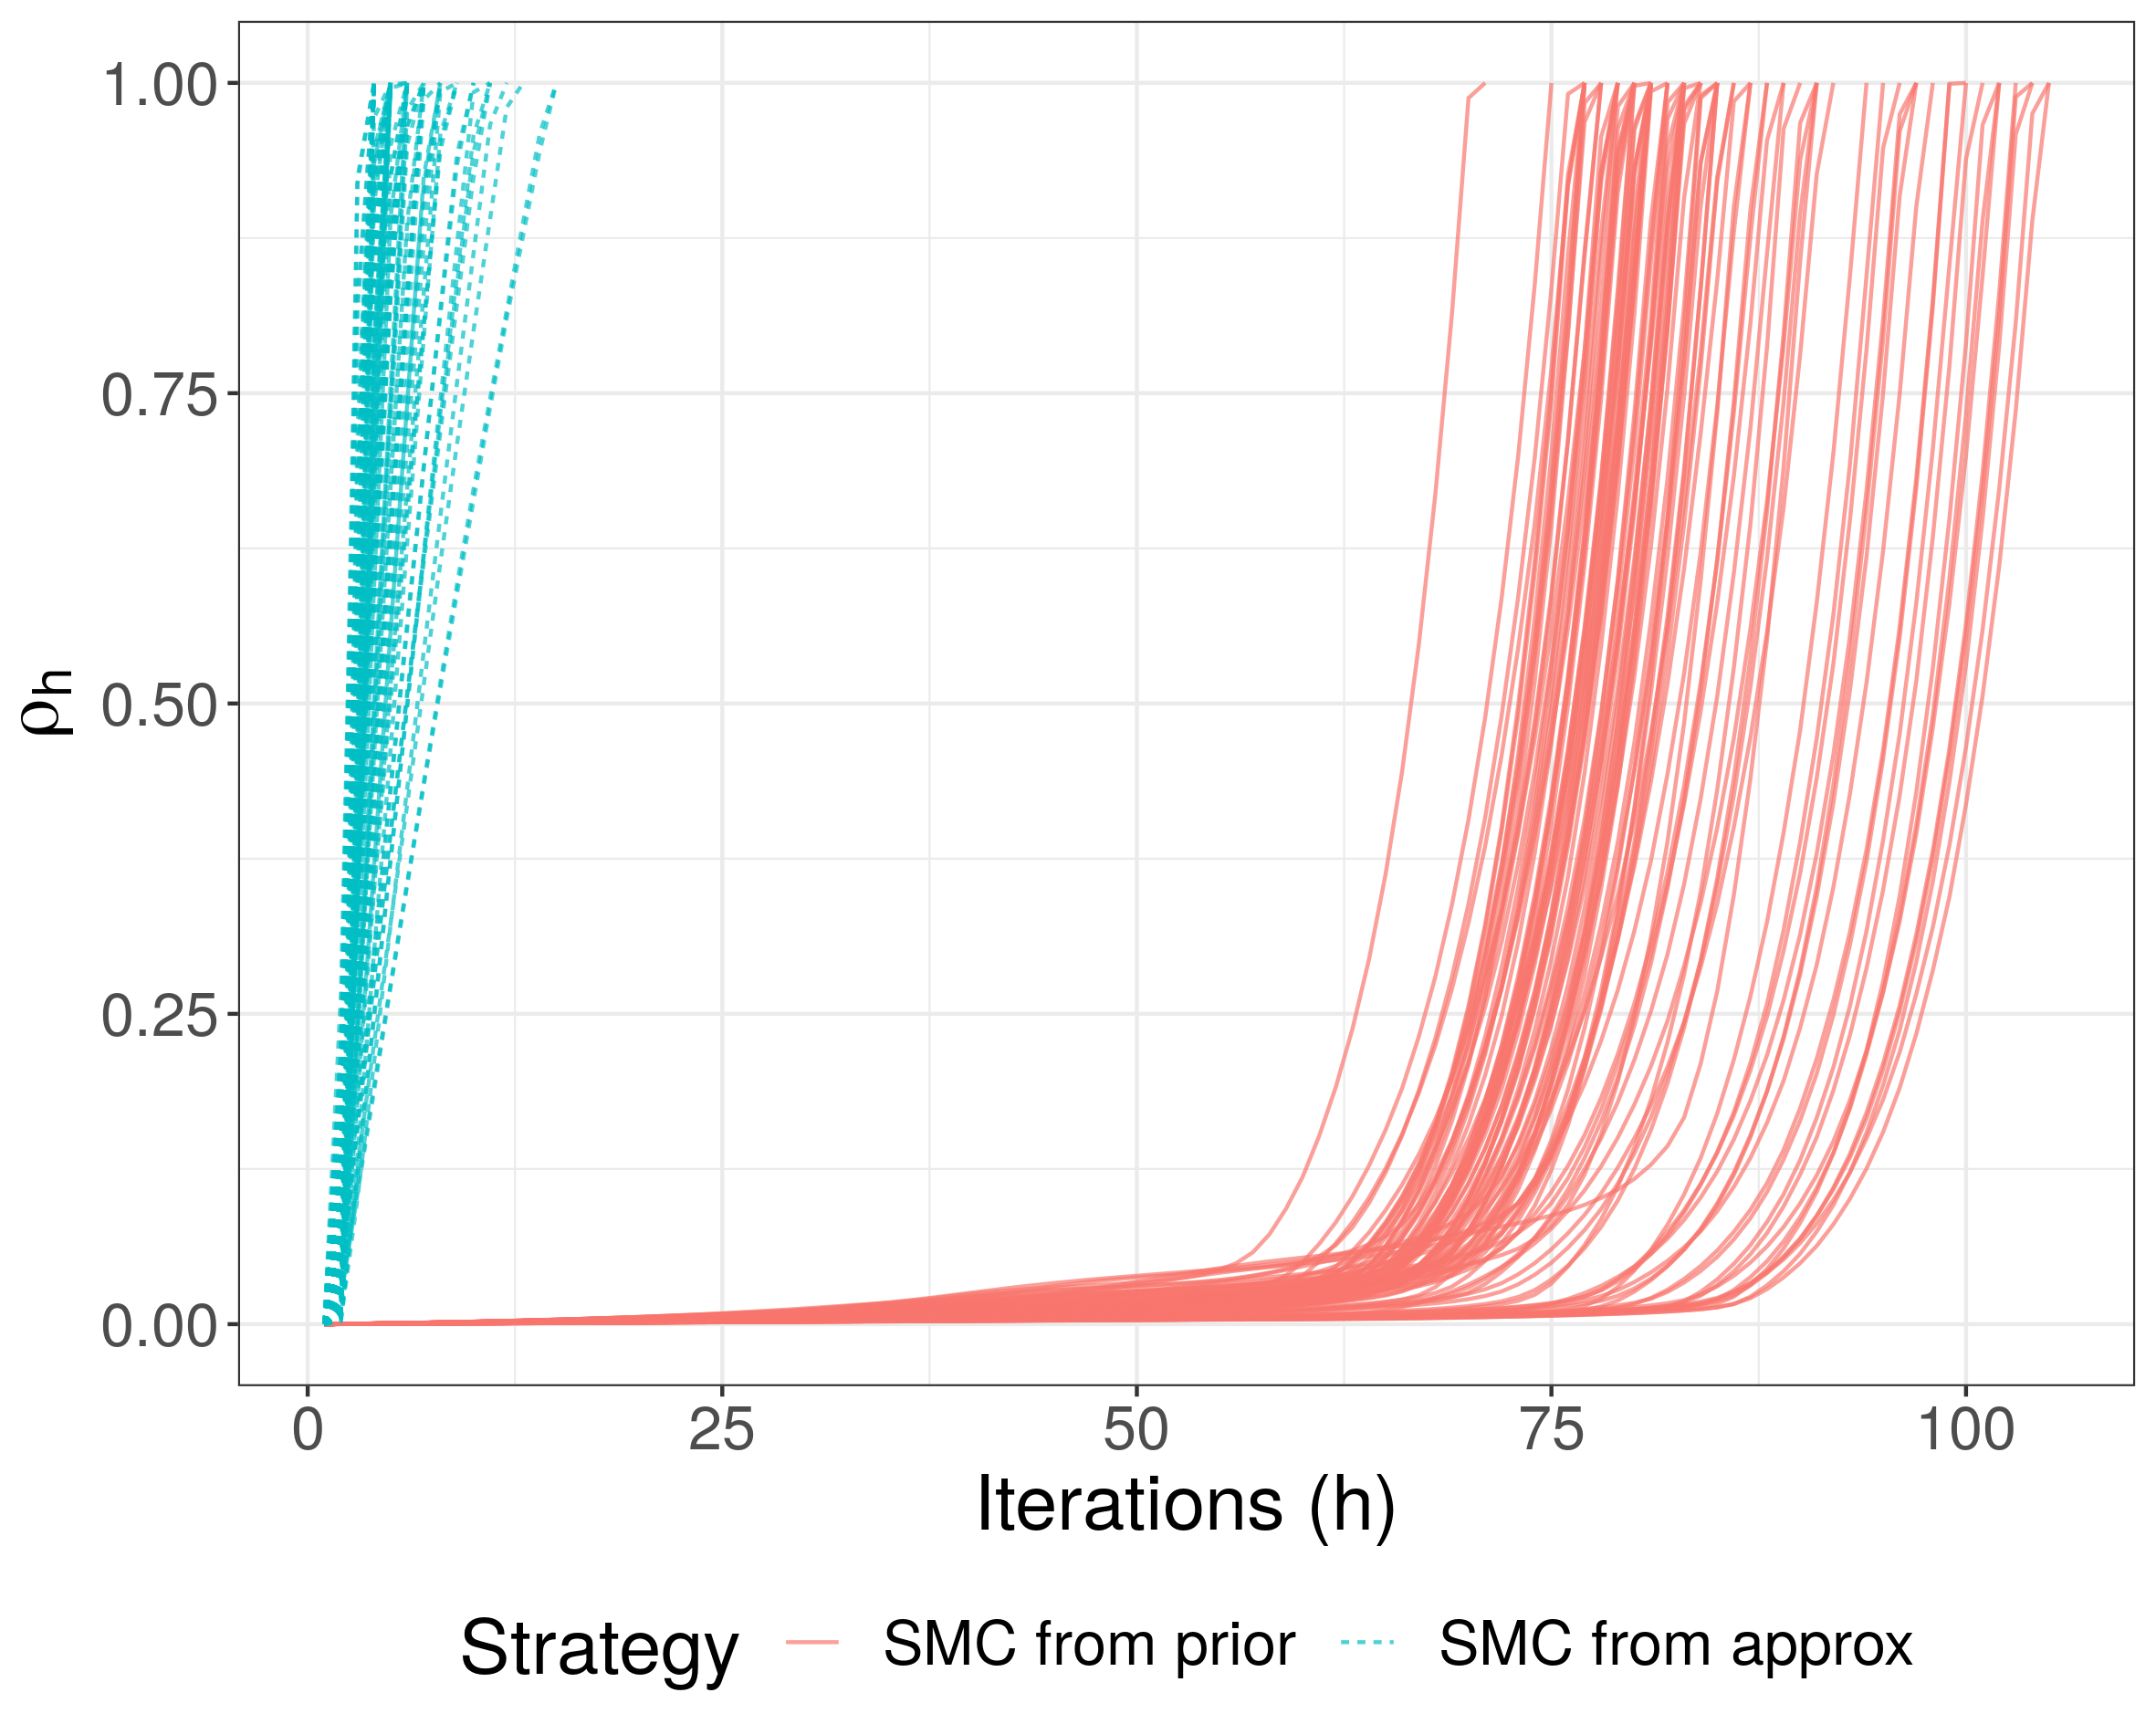
\includegraphics[width=.25\textwidth, height=.21\textwidth, trim=0 20 0 30]{\figDoR/simu_traj_rho} \\
    \rho_h 
    & \displaystyle{KL\left(p_h(Z) \; \| \; \prod_i p_h(Z_i)\right)} 
    & \\
  \end{array}
  $$
  from \refer{DoR19}
  
  \bigskip
  \textcolor{gray}{Back to \#\ref{back:smcPath}}
  
}



%====================================================================
\backupend 

%====================================================================
%====================================================================
\end{document}
%====================================================================
%====================================================================

  \begin{tabular}{cc}
    \hspace{-.04\textwidth}
    \begin{tabular}{p{.5\textwidth}}
    \end{tabular}
    &
    \begin{tabular}{p{.45\textwidth}}
    \end{tabular}
  \end{tabular}

